\documentclass[10pt,twoside,english,a4paper]{article}
%I can write this in English
% Engineering methods

\usepackage{graphicx} % Required for inserting images

%\usepackage[T1]{fontenc}
\usepackage[IL2]{fontenc}
\usepackage[utf8]{inputenc}
\usepackage{url} % block \url for formatting URL
\usepackage{hyperref} %links in text will be active(for some classes of documents makes document shift)
\usepackage{amsmath}
\usepackage{cite}
\graphicspath{{images/}}
\usepackage{wrapfig}
\usepackage{geometry}
%\usepackage{times}
\newgeometry{vmargin = {30mm}, hmargin = {17mm, 17mm}}
\pagestyle{headings}

\AtBeginDocument{%
    \setlength\abovedisplayskip{5pt}%
    \setlength\belowdisplayskip{5pt}%
    \setlength\abovedisplayshortskip{2pt}%
    \setlength\belowdisplayshortskip{2pt}}
\begin{document}


\title{Delivering Relevant Product Recommendations in Finance\thanks{Semester project from subject Engineering methods, academic year 2024/25, management: Martin Sábo}} 

\author{Mykhailo Chepara\\[2pt]
	{\small Slovak Technical University in Bratislava}\\
	{\small Faculty of Information and Information Technologies}\\
	{\small \texttt{xchepara@stuba.sk}}
	}
    \date{\small October 1 2024}


\maketitle

\begin{abstract}
To begin with, why is that topic? 
One of my friends is working in a financing company, therefore I'm genuinely curious how does a bank recommend products to it's customers. As well as how do some systems recommend stock recommendations to investors. It's a useful tool for bank to increase it's revenue. For an investor a significant instrument that can offer good offers on a trade market. Can it be enhanced? And if yes then how?

Now to the points that I'm going to untangle in this article:
\begin{itemize}
    \item What is a recommendation system?
    \item Distribution of the systems based on their category
    \item Usage cases in real life
    \item Architecture and concept of work
    \begin{itemize} 
         \item Architecture and ways of utilizing data
         \item Algorithms applied and models used
         \item Data fetch and processing
    \end{itemize}
    
    \item Conditions to be met before deployment of the system
    \begin{itemize}
        \item Learning conditions
        \item Duration of learning
        \item And other conditions
    \end{itemize}
    
    \item Issues with the system
    \begin{itemize}
        \item Lack of data
        \item New item introduction
        \item Inability to recommend anything relevant to a user
        \item And other issues
    \end{itemize}
    
    \item Enhancement of the system
    \begin{itemize}
        \item Augmentation of one system with another
        \item Systems that can be merged with recommendation system in finance
        \item Other improvements
    \end{itemize}\cite{arch_rec_sys}
\end{itemize}


\end{abstract}
\newpage
\tableofcontents

\begin{figure}[h!]
    \centering
    
\includegraphics[width=1\textwidth]{STU-FIIT-anch}
\end{figure}

\newpage






\section{Recommendation system}

\subsection{Definition of a recommendation system and its objective}
Nowadays, people buy a lot of things on the internet, they watch a lot of films and do a lot of other stuff. Since there's such a rich number of choices, it's hard to find the ones people would choose. For that reason, a recommendation system was introduced. A recommendation system, also called, recommender system, is a program whose main point is to recommend users a product/service which he/she most probably will buy. Ultimately, it tries to predict the next probable choice of a customer and then recommends it. It could be the next film watched, the next purchase bought or the next route on the road recommended. The data is provided from the customer's overall experience. So it's a system, adapting to each customer's needs and preferences.\cite{vars_rec_sys}
\subsection{Recommendation system in Finance}
\par  The system we're going to talk about is a system which recommends offers on stock or any other liquidity markets. Since a lot of people buy stocks to earn money, and a lot of them would be happy to know where prices on the stock market will go, a necessity in finance recommendation systems has appeared. It's hard to predict stock prices: it depends on factors such as inflation, supply, demand, company's state, economic reports, news, investor's sentiment etc. Adding to that probability of factors influencing each other, prices can strongly fluctuate. Offers are chosen according to the certainty of a successful sale. Thus, it's going to be easier to buy and sell them.\cite{stock_rec}\cite{stock_prices}

\subsection{Distribution of the systems based on their category}
The systems are divided into few main categories. Some of them are content-based systems, collaborative systems and hybrid systems. Here is a graph of most famous ones
\begin{figure}[h]
\centering
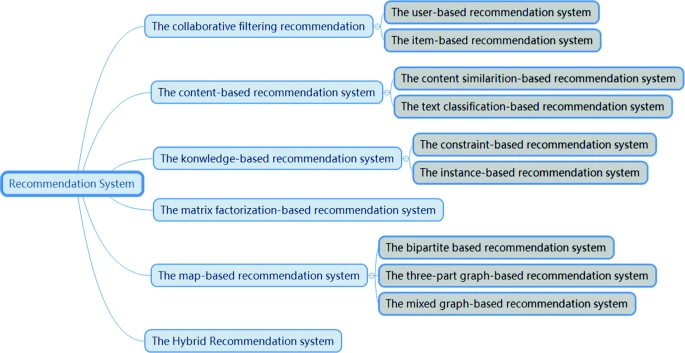
\includegraphics[width=1\textwidth]{system_vars}
\caption{Distribution of systems based on their category}\cite{wang2019review}
\label{fig:System categories}
\end{figure}


Here are the most widely used recommendation systems today.
\par \textbf{Collaborative systems} is one of the most used types of recommendation systems in the world. Collaborative system recommends something based on preferences of another user which has common traits with the current one. Advantages are filtering complex information, recommending completely new information, utilizing feedback of similar users. Disadvantages are rarity of scores, multiple content, scalability.


\par \textbf{Content-based system} is the most used type of system in academic search engines. The plain idea of it is to record which object the user has chosen from the list of recommended products and then analyze it, based on the most relevant object next. For example, academic, fresh attributes. The point is to recommend an object which has the biggest similarity in terms of description to the description provided by the user. Advantages are cold start, ability to adapt to user's preferences, no problem with new objects recommendation. Disadvantages: in case of a user's account deletion, his preferences are gone, it might recommend the same product multiple times, and lack of history. 


\par \textbf{Knowledge-Based Recommendation system} is a type of recommendation system which uses auxiliary information about products and users to give out appropriate results. This kind of recommendation system has an advantage against regular systems are content-based cold start. 
Advantages: history of ratings isn't required, recommendations aren't dependent on user's preferences, so user's data isn't needed. Disadvantages: knowledge acquisition bottleneck, lack of needed information.




\par \textbf{Hybrid-Based Recommendation system} consists of multiple system types which cancel out each other's flaws. It has 7 main strategies for filtering. Here are a few of them.
\par Switching: this method basically selects a recommender system based on its accuracy. Feature combination: ultimately, one system is complemented by features of another. 
Feature Augmentation: each time a new item is recommended, new feature is offered based on which next recommendation is made, so each new recommendation is made using previous features. 
Meta-level: recommendation system uses an input output of another system. 
\subsection{Usage cases in real life}
The main variations of recommendation systems which are most commonly used.

\begin{figure}[h]
\centering
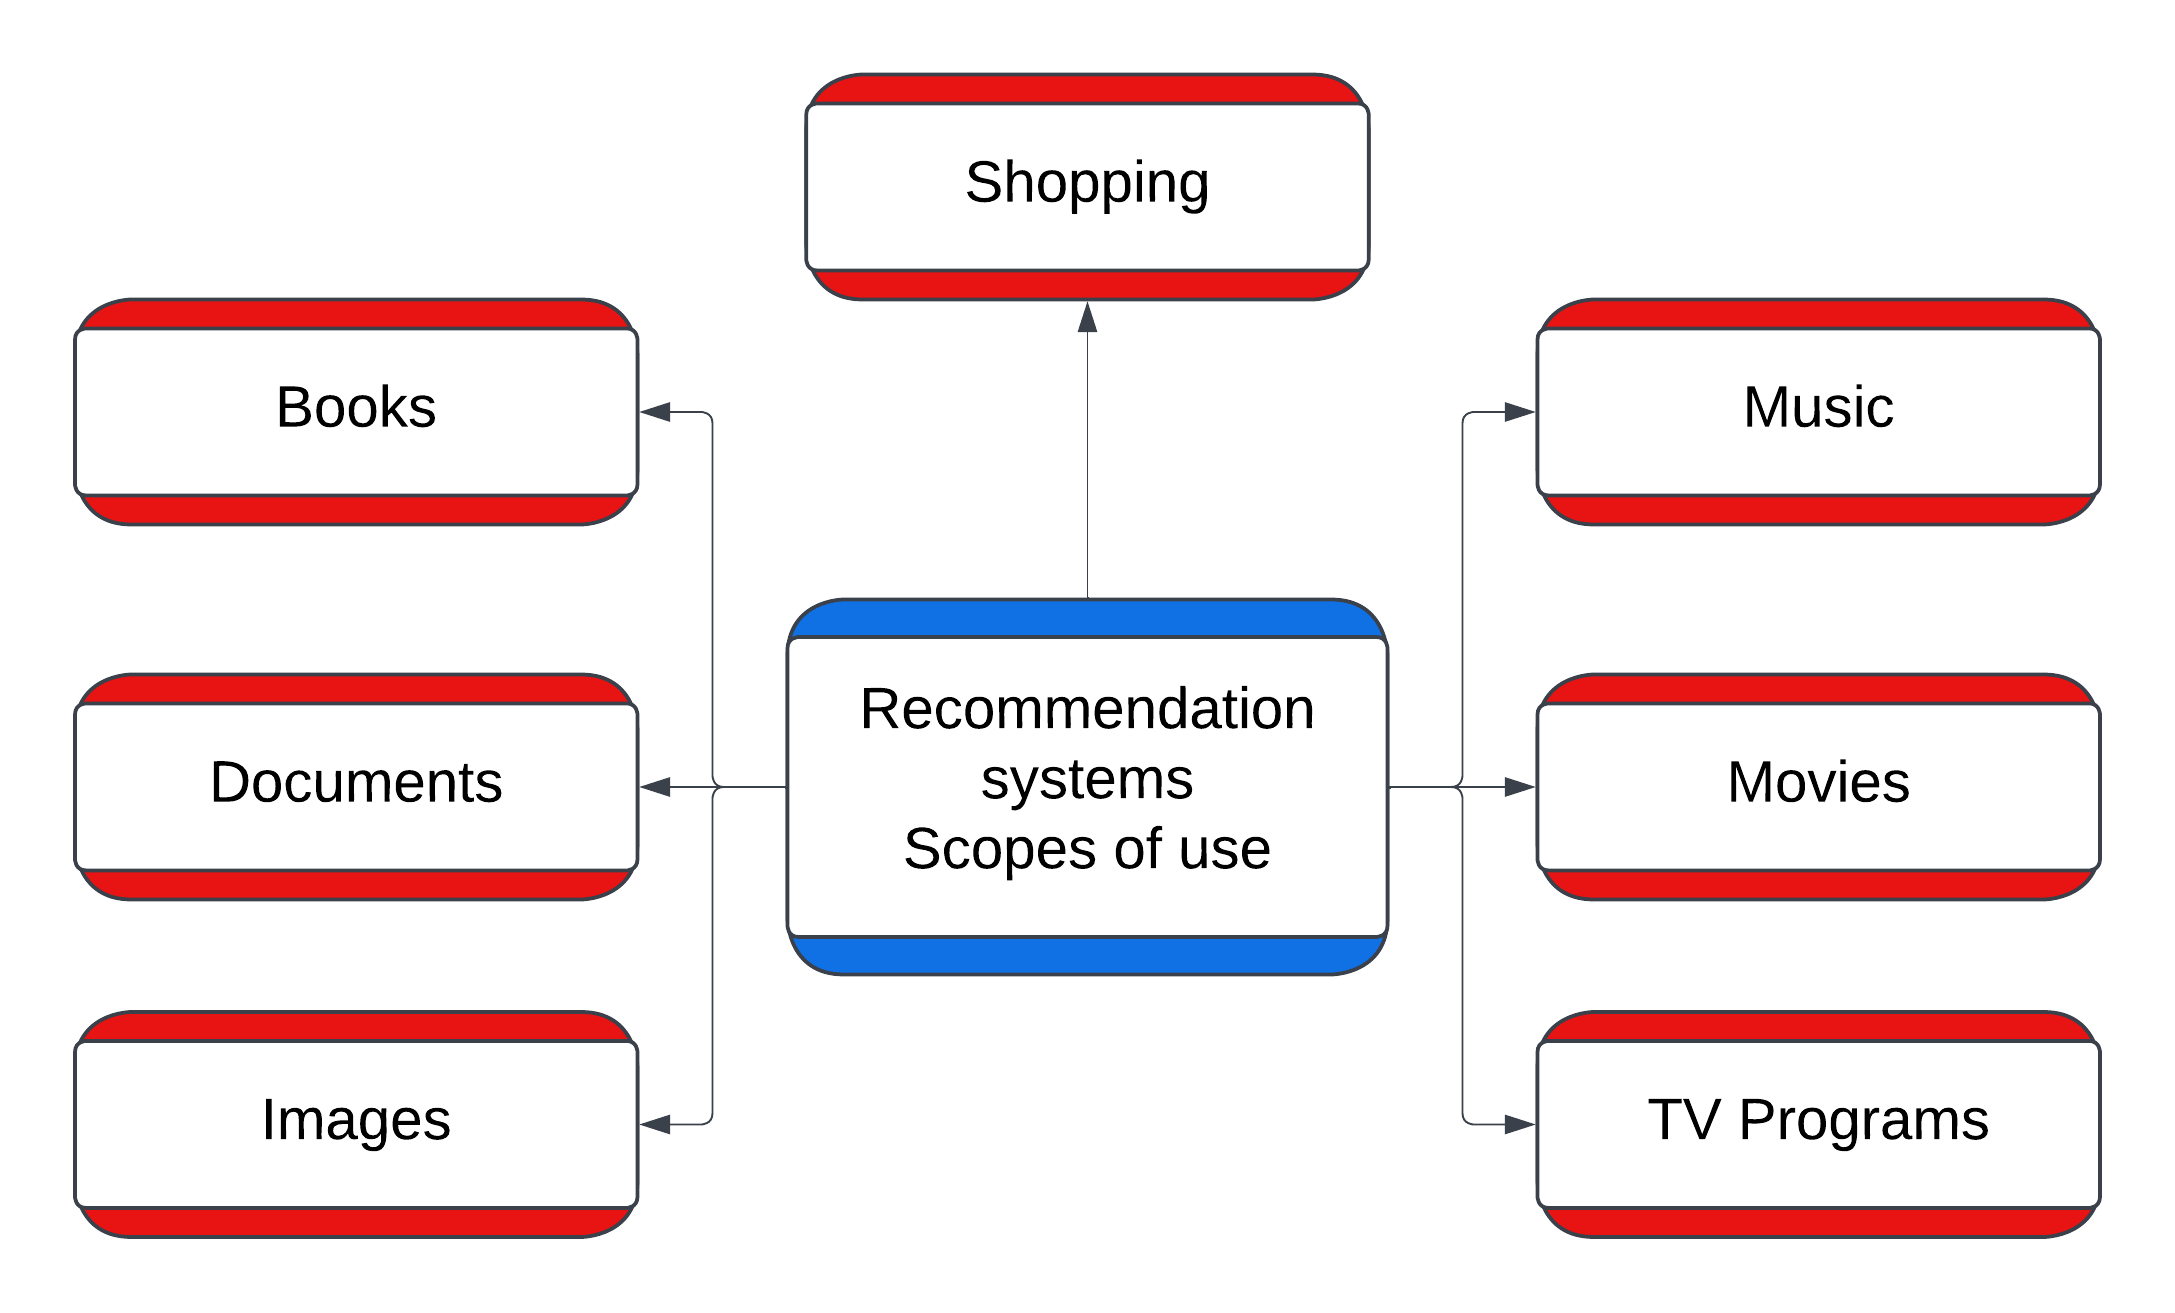
\includegraphics[width=1\textwidth]{system_types}
\caption{Most commonly used system types}
\label{fig:Types}
\end{figure}
\par Spotify, Apple Music, YouTube music and other platforms use recommendation systems to match their user's preferences and show appropriate results for search requests. In that particular field of human art, collaborative filtering and content-based filtering is used in most cases.\cite{music_rec}
\par Google Play Books, Open Library, and Goodreads are apps that manifest the power of recommendation system for recommending books, articles and other handwritten works to their customers. Matrix factorization - collaborative filtering algorithm which is used for this scope as a default decision for recommending desired results.\cite{book_rec}
\par Microsoft Word, Excel, PowerPoint, all of them use file recommendation in order to keep track of important work by recommending files which were frequently edited, commented or people were mentioned in them.\cite{file_rec} 
\par Netflix, Amazon Prime Video, and Hulu use, systems recommendation systems to recommend movies, TV shows and animes to their clients, which increases profits significantly. For example, Netflix reported saving \$1 billion dollars by engaging customers with recommended movies. Techniques of collaborative filtering, content-based filtering, and hybrid filtering are used to generate precise apposite recommendations to a customer.\cite{movie_rec}
\par Amazon, Target and L’Oréal are companies which honed their recommendation systems to the highest possible precision to gain the most revenue. Amazon even made its own personalization system called Amazon Personalize systems applies machine learning algorithms to sort out necessary data and use it for systems. In general, it uses a collaborative filtering method.\cite{shopping_rec}\cite{amazon_recsys}


\section{Architecture and concept of work}
Recommendation system in finance can recommend products as well as it can recommend offers which can lead to revenue of individuals. Here's an overall architecture of system capable of recommending fitting stock recommendations

\begin{figure}[h]
\centering
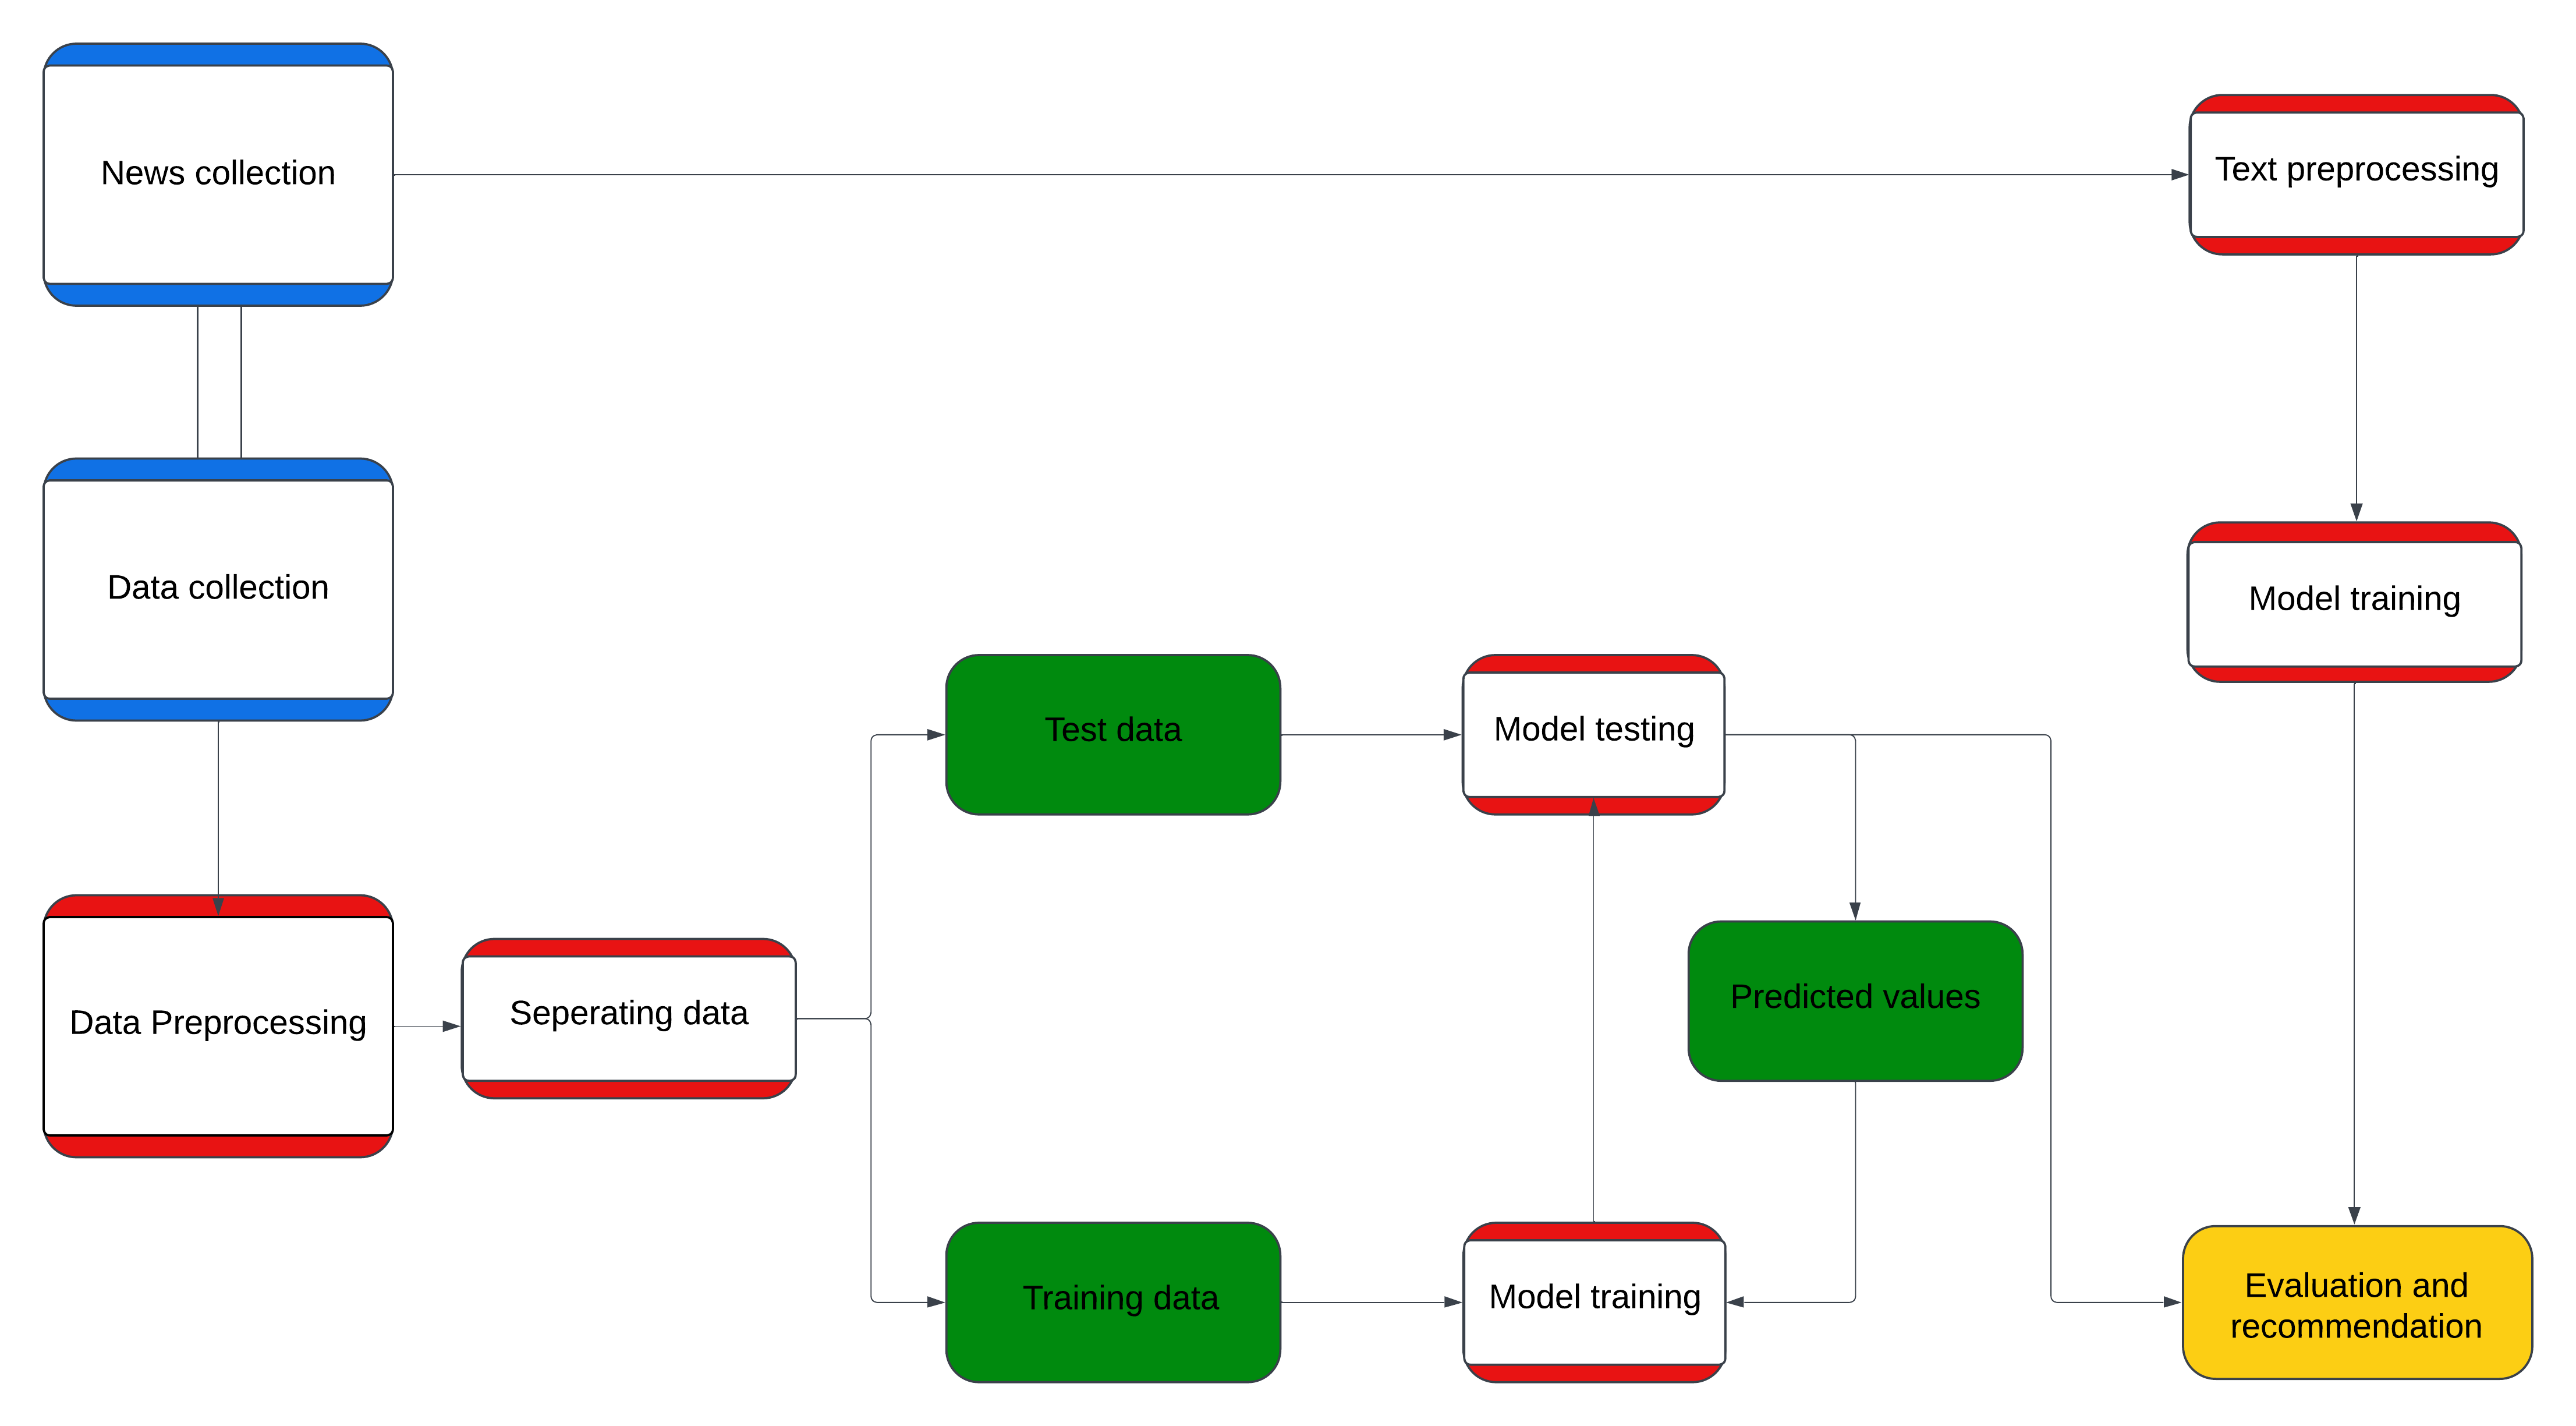
\includegraphics[width=1\textwidth]{architecture_diagram}
\caption{Architecture of finance recommendation system}
\label{fig:Architecture}
\end{figure}

\subsection{Data fetch}
\par In a nutshell, data is collected as a first step. News data is sent into a NLP(Natural Language Processing) preprocessor which decodes sentences and assesses whether news is good or bad. Later conclusion of news processing is used in evaluation of offers. Subsequently, stock market data is analyzed and the conclusion about market volatility is made. Volatility is considered a measurement of the speed at which prices and their ranges change. And then all the data left is separated into training and test data. After which training is made and then, the system recommends the most favorable offers on the market, also including investor's preferences. 
\par Data is collected using API (Application Programming Interface) from trustworthy news sources such as Yahoo Finance, American Stock Market and Alpha Vintage, CNBC, Stock Market and many others.\cite{stock_comp} 
\par Steps for an API to parse data from news websites and stock market data providers. Firstly, it authenticates, uses tokens and API keys to access a website's data, so nobody else will get to it. Then it configures and sends what type of data will be retrieved. Based on the response from the server, it either sends back another request or waits in case of the server being down. Then it receives requested data and saves it into an already existing database.
\subsection{Data processing}
\par Data variables retrieved from stock market providers are: Date, Open, Close, Volume, High, Low, Adjusted close. Percentage Change (Returns) is a crucial variable which predicts how much the price has grown or declined. It measures the volatility of the market. So, to summarize, text data types and number data types are used in calculations for a recommendation. Text obtained from news is preprocessed. Preprocessing consists of a few stages:
\begin{itemize}
    \item Text cleaning, which includes stop word removal, lowercasing words, removing characters, removing numbers, removing unnecessary words.
    \item Normalization is stemming and lemming words. It essentially means to get the root of each word and normalizing words according to their dictionary forms.
    \item Tokenization. Ultimately, it's dividing text into meaningful sections such as paragraphs, sentences or words. In our case, it's words. So each part is called a token.
    \item Feature extraction is achieved by vectorization. Vectorization means that each token is converted into a corresponding numerical value. 
    \item Data transformation. This stage is optional. PCA (Principal, component analysis), t-SNE and UMAP (Manifold Learning), ICP (Independent component analysis), LDA (Linear Discriminant analysis) and other techniques can be used to decrease dimension of feature set matrix.\cite{dimens_red}
    \item Splitting data for analysis. Data is split into training and testing data.\cite{nlp_research1}\cite{nlp_research2}
\end{itemize}
For example, in the article about stock recommendation systems\cite{stock_rec} at the data preprocessing stage there were used methods and algorithms: Stemmer Algorithm, WordNet Lemmatizer, and Stop word removal. After, what data was vectorized using the TF-IDF(Term Frequency Inverse Document Frequency) vectorizer.\cite{stem_alg}\cite{lemm_alg} TF-IDF calculates the tangency value for each word in all the documents in our case datasets. 
Term frequency(TF) is calculated using the formula:
\[ \alpha = \frac{\beta}{\gamma}\]
Where $\alpha$ represents term(word) frequency. $\beta$ is number of occurrences of word in the document and $\gamma$ is total number of words in the document.
\newline
Inverse document frequency(IDF) is calculated using the following formula
\[ \sigma = \log (\frac{\rho}{\epsilon} + 1)\]
Where $\sigma$ represents inverse document frequency value. $\rho$ is total number of documents and $\epsilon$ is number of documents in which our word occurs. 
\newline 
And so the TF-IDF is represented by this formula
\[ TF-IDF = \alpha*\sigma\]
\par Main analysis of the data can be conducted using Random Forest Algorithm, LSTM model and Logistic Regression. Nevertheless, it could be done differently using other ANNs(Artificial Neural Networks) and RNNs(Recursive NEural Networks) complemented by Naive Bayes classifier or SVM(Support Vector Machines).

\subsection{Algorithms and models used}
\subsubsection {Models used to predict prices on the market} 

Now for the data analysis of the stock market dataset. There are lots of models for analyzing and predicting data, but in our case, to foretell prices in such an unpredictable market, sophisticated models are required, which must forecast the volatility of the market. Furthermore, they must know how to work with time series.

Here are some examples of models that can be used for prediction.
\newline\textbf{Statistical models}:
\newline ARIMA(AutoRegressive Integrated Moving Average) models. They work well with a series of data points. By finding, dependency between them, they find the volatility rate of the market.
\newline GARCH(Generalized Autoregressive Conditional Heteroskedasticity) are also used for forecasting market volatility as well as the degree of risk.
\newline
\textbf{Deep learning Models}:
\newline ANN(Artificial Neural Networks) can learn complex relationships and are made of several layers of interconnected points(nodes). But are not suitable for unpredictable market.
\newline RNN(Recurrent Neural Networks) are designed to work with successive data. But they're suffering form vanishing gradient problem
\newline LSTM(Long Short-Term Memory) model is a type of RNN which has resolved the issue of vanishing gradient. It fits the best among models to predict prices.
\newline There are, of course, other model types, but we'll stop on the LSTM model, since it's the most efficient and suited for our purpose. 
\newline
\newline LSTM model is made of three main parts named gates. Input gate, forget gate and output gate. All the gates control the flow of information. Information is splitted into cells and hidden states. Cell state represents the long-term memory. The hidden state represents short-term memory. Gates are used to forget, save and update information throughout the period of learning. 
\newline Forget Gate: 
\[f_{t} = \sigma (W_{f}*[h_{t-1}, x_{t}] + b_{f})\]
$W_{f}$ and $b_{f}$ are weights and bias of the forget state. $f_{t}$ is the output of the forget state. If it's close to 0 it's forgotten if close to 1 it's remembered. $h_{t-1}$ is previous short-term memory value. $x_t$ is current input value(record)
\newline Input Gate:
\begin{align*}
    i_{t} = \sigma(W_{i} * [h_{t-1}, x_{t}] + b_{i}) \\
    \Tilde{C_{t}} = \tanh{W_{C}*[h_{t-1}, x_{t}] + b_{C}}
\end{align*}
$i_t$ determines whether to remember or not the value of the new input. $C_t$ is value for the new input.
\newline Cell state update:
\begin{align*}
    C_t &= f_t * C_{t-1} + i_t * \tilde{C}_t \\
\end{align*}
$C_t$ is new long-term memory $f_t$ is forget gate, $C_{t-1}$ is previous long-term memory and $i_t$, $C_t$ are values from input gate.
\newline Output gate:
\begin{align*}
    o_t &= \sigma(W_o \cdot [h_{t-1}, x_t] + b_o) \\
    h_t &= o_t * \tanh(C_t)
\end{align*}
$h_t$ is output of an entire LSTM unit and is called new short-term memory. Whereas $o_t$ decides whether to keep that new memory or discard of it.
\section{Conditions to be met before deployment of the system}
\subsection{Data quality}
Before deploying the system we need to make sure that it's trained on flawless dataset.The necessity is to have up-to-date legitimate data from trustworthy stock market data providers. Since our model trains on data from dataset it's crucial to include all important features which are Date, High, Low, Open, Close, Volume, Adj. Close.\cite{data_quality}
\subsection{Proper data preparation}
Data preprocessing is as important as model training. First of all data outliers will be either eradicated or filled out with mean, zero or otherwise interpolated with any other value responding to rows' type of values. Then set of techniques is applied to make data easier to compute. Those techniques are standardization, normalization and anomalies detection.
Standardization is fundamentally refactoring our data to one format, e.g divide it onto High, Low, Open, Close, Volume variables. Now model has only one type of dataset to work with, so it's hastier and easier to train. By detecting anomalies we're deleting corrupted data points, which are beyond recovery, and outliers which bring noise i.e inaccuracy to out prediction. Normalization is data scaling which is especially useful in our case because LSTM models are highly sensitive to acute value change spikes.\cite{data_preproc_feature_sel_time_updates}
\subsection{Feature selection}
Feature selection is the next step of preparing data for our model. Here are some methods used to select features for our model, which will reduce learning time and induce accuracy.
Filtering methods spot correlations between features and eliminate uncorrelated ones. Those are Pearson correlation, ANOVA F-test, and chi-square and others. PCA(Principal Component analysis) reduces dimensions by finding covariance between each variable and then selecting those principal components(variables) which have the strongest correlation, leaving behind others.
\cite{data_preproc_feature_sel_time_updates}
\subsection{Timely Data Updates}
Real-time data updates are crucial to any stock recommendation system, which can only be used to capture current market situation. Many of these systems make use of live APIs from services like Alpha Vantage. A system is likely to make better recommendations if it is trained on consistently updated models, because market conditions can oscillate rapidly.\cite{up-to-date_data}
\subsection{Learning duration}
Learning duration depends on few factors, which are model complexity, size and type of data, data preprocessing and training approach. Of course there are more factors but we'll talk about plain ones. The more complex model is the longer it trains.  Models like linear regression, logistic regression can train relatively quickly, even on large datasets. Advanced machine learning models like Random Forests, Gradient Boosting Machines (e.g., XGBoost), and neural networks (LSTM, CNN, Transformer models for time series) have more parameters and thus take longer to train. If model is trained on data hourly than it's always up-to-date with newest data, on the other side is periodic training where model is trained between certain periods of time. Also if data is unstructured it generally takes more time to train model since it's hard to work with sentimental data. 
Here's a table of model training time based on model type
\begin{center}
\begin{tabular}{|c | c|} 
 \hline
 Model Type & Training duration\\ [1ex] 
 \hline\
 Simple Models & Seconds to minutes \\ [1ex] 
 \hline
 Tree=based models& Minutes to hours\\ [1ex]
 \hline
 Basic Neural Networks & Hours\\ [1ex]
 \hline
 Advanced neural networks & Hours to days\\ [1ex] 
 \hline
 Ensemble models & Hours to days\\ [1ex]
 \hline
\end{tabular}
\end{center}\cite{train_t}
\section{Issues with the system}
\subsection{Data quality and availability}
Data gaps and inaccuracies is one of the most occurred problems with datasets since it's not always possible to preserve all data at once, some records can be missing. The next big problem is lag in data flow. It's not always possible to have continuous data updates throughout period of learning. Because of delays model doesn't have all the features updated from the same time period, so inexactitude appears.\cite{quality}
\subsection{Overfitting to Historical Data}
If model overfits to historical data it applies same measurements of features which were relevant in the past, hence it forecasts wrong value. Additionally, stock market is highly volatile and even without overfitting to historical data it's hard for model to get used to new patterns after rapid change. The predicted price is significantly dependent on previous data outliers in this case.\cite{overfit}
\subsection{Scalability and Computational Demands}
In order to process high-frequency data in real-time, large amount of computational power is required. It becomes even harder when data has different structure and needs prior preprocessing. So to complete all that either cloud computing is used or manual power station is needed to fulfill all demands. Not only that it's expensive to use cloud computing, since data needs to be secured as well.\cite{scalability}
\subsection{Model Complexity and Interpretability}
The more complex the model is the harder it is to understand which operations it does per one iteration. From that emerges the problem of interpretability. When model crashes we can't deduce why, thus we're unable to look through each step it does.\cite{complexity}
 
\section{Enhancement of the system}
\subsection{Integration of Diverse Data Sources}
Using news in real-time and articles, social media, forums for sentiment analysis can capture market events influencing stock movement. Regular updates allow models to capture the latest trends, reducing errors caused by outdated data. This is particularly significant for time-sensitive models like LSTMs and XGBoost. Models working with updated data all the time can respond to sudden changes in market.\cite{diverse_datsrc}
\subsection{Improving Data Preprocessing Techniques}
Techniques such as moving averages, exponential smoothing, or wavelet transformations can help minimize price noise and show the underlying trends.
For sentiment analysis on textual data, consider using advanced transformer models like BERT or GPT to catch subtle shifts in news related to stock market.
Create automated pipelines for real-time data cleaning to quickly find outliers, missing values, or erroneous data points, making sure there's minimal disruption to the model's performance.
\subsection{Incorporating Adaptive Learning and Model Retraining}
Models can be either trained periodically on huge data sets and be insensitive to shifts stock market. Or trained continuously on data. being able to predict with high accuracy current price. because overtime features change their correlation consistent training mus be applied in order to address the problem.\cite{adaptive_learning} 
\subsection{Reinforcement one system's cons with another system's pros}
Reinforcement learning models are often used with temporal models such as CNN (Convolutional Neural Networks) to find trends and reduce noise, which improves forecasting. Reinforcement learning used with supervised learning is one of the possibilities to improve model. Reinforced-learning model enhances decisions from feedback from the environment. Next possibility is statistical models used with machine learning models. Here statistical models predict price while machine learning models detect complex patterns to provide more accurate results.\cite{reinfocment}
\subsection{Systems adept to complement each other}
 (RL) Reinforcement Learning with Supervised Learning can improve prediction accuracy. Examples of reinforcement models capable of complementing main prediction model are (DQN) Deep Q-Networks, (PPO) Proximal Policy Optimization, Actor-Critic Models etc. Supervised learning establishes basic prediction, after what reinforcement model adapts to changes on of the market in real time to optimize decision-making. Examples of supervised learning models: Random Forest, (SVM) Support Vector Maxchines, Logistic Regression etc.
 \par Blending statistical methods like ARIMA with machine learning algorithms (XGBoost). This works particularly good with volatile markets since ML models search for intricate patterns and then it makes a prediction based on those patterns. Examples of statistical models: (ARIMA) AutoRegressive Integrated Moving Average, (SMA) Simple Moving Average, (EMA) Exponential Moving Average, Facebook Prophet etc. As for deep learning models could be Long Short-Term Memory (LSTM), (GRU) Gated Recurrent Unit etc. \cite{adept_sys}\cite{adept_sys1}\cite{adept_sys2}\cite{adept_sys3}

\newpage
\bibliography{literature}
\bibliographystyle{plain}

%Shcolar - https://link.springer.com/chapter/10.1007/978-981-13-7025-0_34
%Scolar - https://www.sciencedirect.com/science/article/pii/S0957417412002825#f0005 
\end{document}
